\documentclass{beamer}
\usepackage{lipsum}
\usepackage[brazilian]{babel}
\usepackage[utf8]{inputenc}

\usepackage{enumerate}
\usepackage{dcolumn}
\usepackage{tabu}
\usepackage{colortbl}
\usepackage{booktabs}
\usepackage{changes}
\usepackage{listings}
\usepackage{placeins}
\usepackage{amsmath}

\usepackage{multirow}

\newcommand*{\Scale}[2][4]{\scalebox{#1}{$#2$}}%
\newcommand*{\Resize}[2]{\resizebox{#1}{!}{$#2$}}%

\usetheme[faculty=ppca,language=logo,framenumber,totalframenumber]{UniversiteitGent}

\title{Implantando o barramento de serviços ERLANGMS no CPD/UFSM}
\subtitle{ \textcolor{black}{Universidade Federal de Santa Maria} \\
			\textcolor{black}{\small{Centro de Processamento de Dados}} 
}



\author{Everton de Vargas Agilar (UnB / UFSM) \\
		Jader Adiel (UFSM)
}



\begin{document}

\begin{frame}
  \titlepage
\end{frame}




%%##################### PLANO #########################################

\section{Plano}


\subsection{Plano}

\begin{frame}
  \frametitle{Plano}

    \begin{itemize}

	    \item<1-> Barramento de serviços ERLANGMS
		    \begin{itemize}
		  	  \item<1->Objetivo do projeto
		  	  \item<1->Panorama geral sobre modernização
	    	  \item<1->Histórico do projeto
  	  	 	  \item<1->Design da arquitetura
		    \end{itemize}
	   	  \item<1-> 

	    \item<1-> Implantação do barramento na UFSM
		    \begin{itemize}
			\item<1->O que está sendo feito
			\item<1->Desafios da migração do backend Delphi para Java
			\item<1->Plano de desenvolvimento da versão 2.0
			\item<1->Caso prático 1: Web services implementados para o NCC
			\item<1->Caso prático 2: TClis do SIE invocando web services Java
		    \end{itemize}
   	    \item<1-> 
   	    


	 \end{itemize}	   	  

\end{frame}



%%##############################################################


\section{Barramento de serviços ERLANGMS}


\begin{frame}[c]{ }
\centering
\huge{Barramento de serviços ERLANGMS}
\end{frame}


\subsection{Objetivo do projeto}


\begin{frame}
\frametitle{Objetivo do projeto}

\begin{exampleblock}{ERLANGMS}
	
	É uma abordagem desenvolvida na UnB para facilitar a modernização de sistemas para uma arquitetura orientada a serviços 
	por meio de um barramento de serviços + SDK + processo 
	de modernização e arquitetura documentado (SMSOC).
	
\end{exampleblock}


\end{frame}



\begin{frame}
\frametitle{Panorama geral sobre modernização  \\ \small{Estudo realizado para identificar as estratégias de modernização}}

%% Mostra o diagrama de bolhas

	\centering
	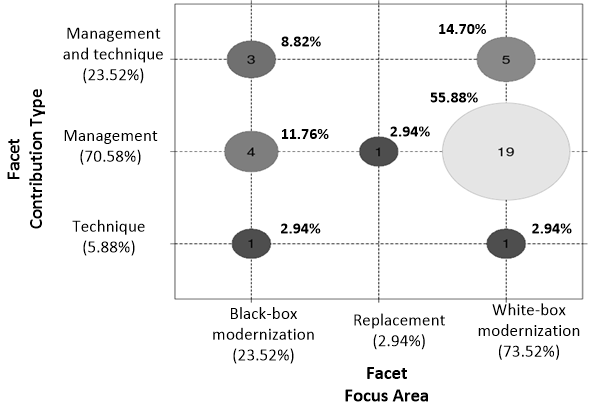
\includegraphics[scale=0.45]{img/bubble_diagram.png}

\end{frame}


\begin{frame}

	\frametitle{Histórico do projeto}

	\centering
	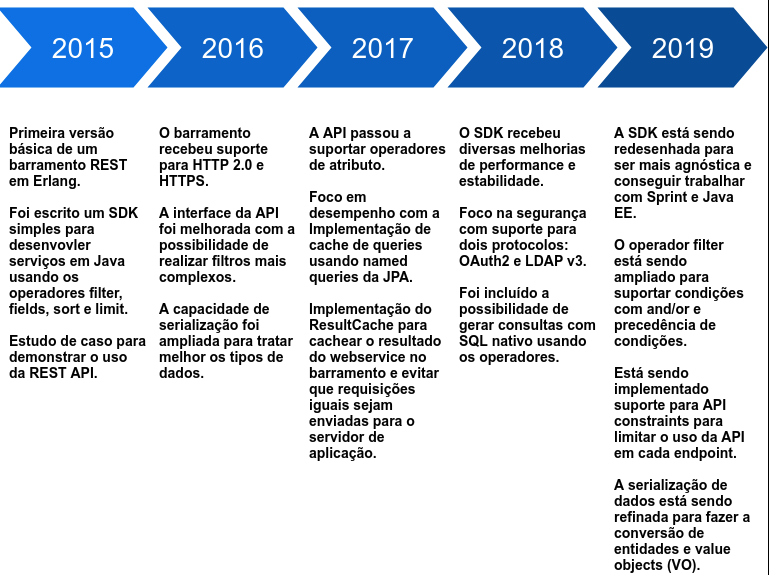
\includegraphics[scale=0.30]{img/historico.png}

\end{frame}



\begin{frame}
	\frametitle{Histórico do projeto \\ \small{Principais features em uso na UnB}}

\begin{exampleblock}{Features}
	
	\begin{itemize}
		\item<1->HTTP/2, HTTP/1.1, HTTPS (Secure TLS Listener);
		\item<1->LDAP v3 -- Proxy LDAP;
		\item<1->HTTP Basic authentication;
		\item<1->OAuth2 authentication;
		\item<1->SDK para criar serviços em Java;
		\item<1->Query Api -- filter, fields, sort, limit.
		\item<1->Suporte para Dados Abertos.
	\end{itemize}
	
\end{exampleblock}


\end{frame}




\begin{frame}
\frametitle{Design da arquitetura}

\begin{exampleblock}{Design da arquitetura}
	
	\begin{itemize}
		\item<1->Multiplataforma e arquitetura modular;
		\item<1->Serviços especificados em catálogos de serviços;
		\item<1->Cluster de serviços para evitar ponto único de falhas;
		\item<1->Suporta serviços RESTful por contrato;
		\item<1->Modelo de concorrência para serviços em Erlang: Actor Model;
		\item<1->Baixa curva de aprendizado.
	\end{itemize}
	
\end{exampleblock}


\end{frame}




%%##############################################################






\section{Implantação do barramento na UFSM}


\section{Implantação do barramento na UFSM}


\begin{frame}[c]{ }
\centering
\huge{Implantação do barramento na UFSM}
\end{frame}




\begin{frame}
\frametitle{O que está sendo feito}

\begin{exampleblock}{O que já foi feito}
	
	\begin{itemize}
		\item<1->Implantação do barramento em partes, priorizando:
			\begin{itemize}
				\item<1->Query API
				\item<1->Subsistema de serialização;
				\item<1->Adaptar a interfaces do SDK para trabalhar de forma agnóstica com Java EE e Spring. 
			\end{itemize}
		\item<1->Features visando a migração de backends SIE para Java:
			\begin{itemize}
				\item<1->Novo operador \em{format} para serializar dados como Dataset;
				\item<1->Novo subsistema provider no SDK para permitir seu uso independente da camada de negócio;
				\item<1->Provider para trabalhar com meta-queries do Delphi;
				\item<1->Cliente REST implementado no Delphi.
			\end{itemize}
		
	\end{itemize}
	
\end{exampleblock}


\end{frame}



\begin{frame}
\frametitle{O que ainda precisa ser feito x prioridade}

\begin{exampleblock}{O que ainda precisa ser feito}
	
	\begin{itemize}
		\item<1->Tornar a camada de fachada mais simples -- Moderado;
		\item<1->Implementar o subsistema de autenticação OAuth2 (ou integrar o barramento que já possui) -- Alto;
		\item<1->Analisar os principais métodos do TCliBusiness e prover um suporte adequado no SDK para facilitar a migração -- Alto;
		\item<1->Permitir gerar uma consulta por meio da Query API para buscar dados de um atributo lista de um objeto principal -- Baixo;
		\item<1->Permitir encadear funções nos atributos das entidades com o operador \% para modificar a forma como o dado é lido da fonte de dados -- Baixo.
		
		
	\end{itemize}
	
\end{exampleblock}







\end{frame}




\begin{frame}
\frametitle{Desafios da migração do backend Delphi para Java}

\begin{exampleblock}{Desafios da migração do backend Delphi para Java}
	
	\begin{itemize}
		\item<1->Basicamente, qualquer parte do Delphi é um desafio enorme levando em consideração o custo de tempo e complexidade do código;
		\item<1->A única excessão será as meta-queries que serja bem fácil com o provider de meta-query do SDK;
		\item<1->Os métodos das TClis possuem muito herança de código com muitos métodos virtuais que dificulta extrair a lógica de negócio
		sem precisar refazer tudo no Java;
		\item<1->Para mapear os dados em Dataset, é necessário especificar o schema dos Dados;
	\end{itemize}
	
\end{exampleblock}

\end{frame}


%%##############################################################



\section{Principais Resultados do Trabalho}


\begin{frame}[c]{ }
\centering
  \huge{Principais Resultados do Trabalho}
\end{frame}



\begin{frame}
  \frametitle{Desenvolvimento de serviços com o SDK}

	\begin{figure}
	\centering
		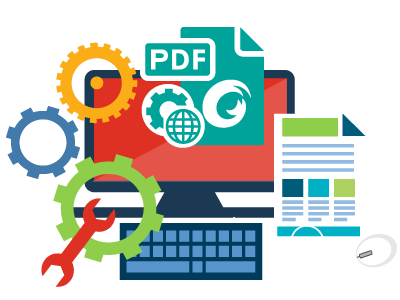
\includegraphics[scale=0.4]{img/sdk.png}
	\end{figure}
  
\end{frame}


\begin{frame}
  \frametitle{Autenticação de usuários com o proxy LDAP}

	\begin{figure}
	\centering
		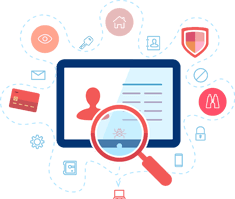
\includegraphics[scale=0.6]{img/ldap.png}
	\end{figure}
  
\end{frame}


\begin{frame}
  \frametitle{Autenticação e autorização de serviços REST com OAuth2}

	\begin{figure}
	\centering
		
\includegraphics[scale=0.4]{img/oauth2.png}
	\end{figure}
  
\end{frame}



\begin{frame}
  \frametitle{Trabalhos futuros}

  \begin{exampleblock}{Trabalhos futuros}
  
	  \begin{itemize}
 	    \item<1->Portal Api Management;
    	    \item<1->JSON Schema Draft 4;
    	    \item<1->SDK .Net.
	  \end{itemize}

  \end{exampleblock}

  
\end{frame}


%%##############################################################


\subsection{Perguntas}


\begin{frame}[c]{ }
\centering
  \huge{Perguntas ?}
\end{frame}


\begin{frame}
  \frametitle{Perguntas}

  \begin{exampleblock}{}
  
	  \begin{itemize}
		\item<1->(QP1) Por que Erlang/OTP?
		\item<1->(QP2) Quem usa Erlang/OTP?
	    \item<1->(QP3) Por que o desenvolvimento de um novo barramento em vez de utilizar um existente?
	    \item<1->(QP4) Por que não implementar web services usando somente Java e seus frameworks?
	  \end{itemize}
  
  \end{exampleblock}

  
\end{frame}


\begin{frame}
  \frametitle{(QP1) Por que Erlang/OTP?}

    \begin{itemize}
       \item<1-> Suporta aplicações distribuídas e tolerantes a falhas a serem executadas em um ambiente de tempo real e ininterrupto;
       \item<1-> Possui um ambiente de execução que realmente facilita o desenvolvimento de software de rede e de clusters de serviços;
       
       \item<1-> Possui um modelo de arquitetura baseado em atores (Actor Model) onde os processos podem 
       se comunicar apenas por mensagens.
       
    \end{itemize}
  
\end{frame}


\begin{frame}
  \frametitle{(QP2) Quem usa Erlang/OTP?}

	  \begin{itemize}
		\item<1->Facebook (Backend do chat -- 100 milhões de usuários ativos);
		\item<1->Whatapps (Servidores de mensagens -- 2 milhões de usuários/servidor);
		\item<1->Yahoo (Delicious -- 5 milhões de usuários e mais de 150 milhões de bookmarks);
		\item<1->Amazon SimpleDB, o serviço de dados do Amazon EC2;
		\item<1->GitHub (Backend -- milhares de transações concorrentes);
		\item<1->T-Mobile nos seus sistemas de SMS e autenticação;
		\item<1->Motorola, CouchDB, RabbitMQ, Ejabbed, entre outros.
						
	   \end{itemize}
  
\end{frame}


\begin{frame}
  \frametitle{(QP3) Por que um novo barramento?}

	  \begin{itemize}
		\item<1->Obter domínio sobre as tecnologias e o design RESTful;
		\item<1->Barramento de serviços são produtos caros e complexos;
		\item<1->Disponibilizar um produto simples (contém somente 10 mil linhas de código atualmente).
					
	   \end{itemize}
  
\end{frame}


\begin{frame}
  \frametitle{(QP4) Por que não implementar web services em Java com frameworks?}

	  \begin{itemize}
		\item<1->É uma opção, mas exige ferramentas para gerenciar;
		\item<1->Não é orientado a contrato de serviços;
		\item<1->Não é independente de linguagem de programação;
		\item<1->Não é escalável apenas usando os frameworks.
	   \end{itemize}
  
\end{frame}



\begin{frame}[c]{ }
\centering
  \huge{Obrigado!}
\end{frame}


\end{document}



